\documentclass{beamer}
\usepackage{lmodern}
\usepackage{subcaption}
\usepackage{caption}
%\setbeamertemplate{footline}[page number] % Fußzeile entfernen und durch Folien-Zahl ersetzen
\setbeamertemplate{navigation symbols}{} % Navigations-Symbole entfernen

\usepackage[utf8]{inputenc} %deutsche Umlaute
\usepackage[ngerman]{babel} %deutsche Sprache
\usepackage{graphicx} %für Bilder
\usepackage{booktabs} %für \toprule \midrule \bottomrule in Tabellen

\usetheme{Ilmenau}
\title{Börsengang von Snap}
\institute{Alex Dudin, Hendrik Schick, Andre Hildebrandt}
\author[]{HTWK Leipzig} %<= used the short author name [] for the footline: leave it blank to not displayed

\begin{document}
\begin{frame}
\titlepage
\end{frame}

\begin{frame}
\frametitle{Inhalt}
\tableofcontents
\end{frame}

\section{Einleitung}




\section{Hauptteil}


\subsection{Börsengang allgemein}

\begin{frame} {Börsengang allgemein}
\begin{figure}
	\centering
	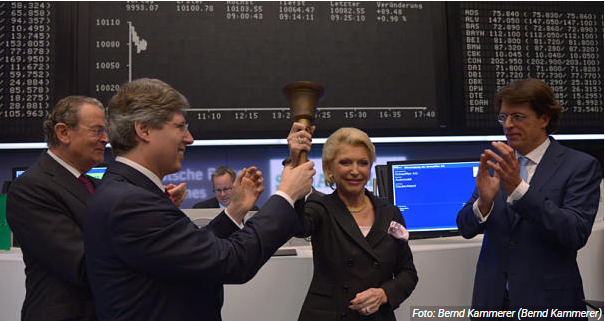
\includegraphics[width=10cm, height=8cm]{boersenglockeeinfuehrung.PNG}
\end{figure}
\end{frame}

\begin{frame} {Was ist ein Börsengang?}
\begin{itemize}
\item Notierungsaufnahme der Aktien eines Unternehmens an bestimmter Börse 
\item Erstplatzierung (englisch "Initial Public Offering" (IPO)) wenn Aktien von Altaktionären oder aus Kapitalerhöhung angeboten werden
\item ansonsten "kalter Börsengang" bloße Notierungsnahme, die oft nur im Freiverkehr erfolgt
\item wird in Regel von einer oder mehreren Investmentbanken vorgenommen
\end{itemize}
\end{frame}

%\begin{frame} {Börsengänge in Deutschland 1990 bis 2017}
%\begin{figure}
%	\centering
%	\begin{subfigure}
%		\left
%		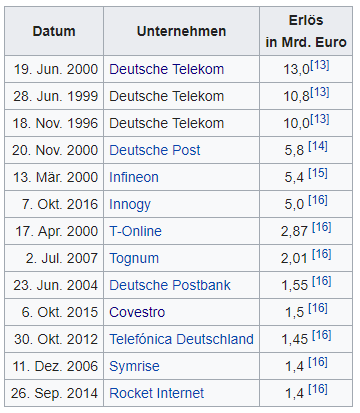
\includegraphics[width=5cm, height=6cm]{groessteBoersengaengeDeutschland.PNG}
%	\end{subfigure}
%	\begin{subfigure}
%		\right
%		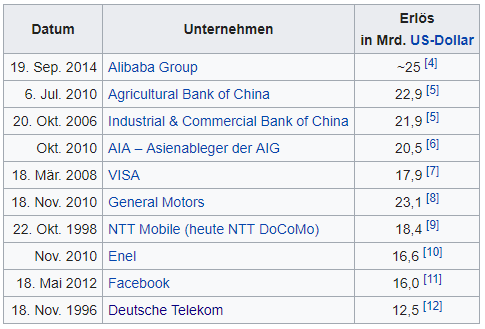
\includegraphics[width=5cm, height=6cm]{groessteBoersengaengeWeltweit.PNG}
%	\end{subfigure}
%\end{figure}
%\end{frame}

\begin{frame} {Börsengänge in Deutschland 1990 bis 2017}
\begin{figure}
	\centering
	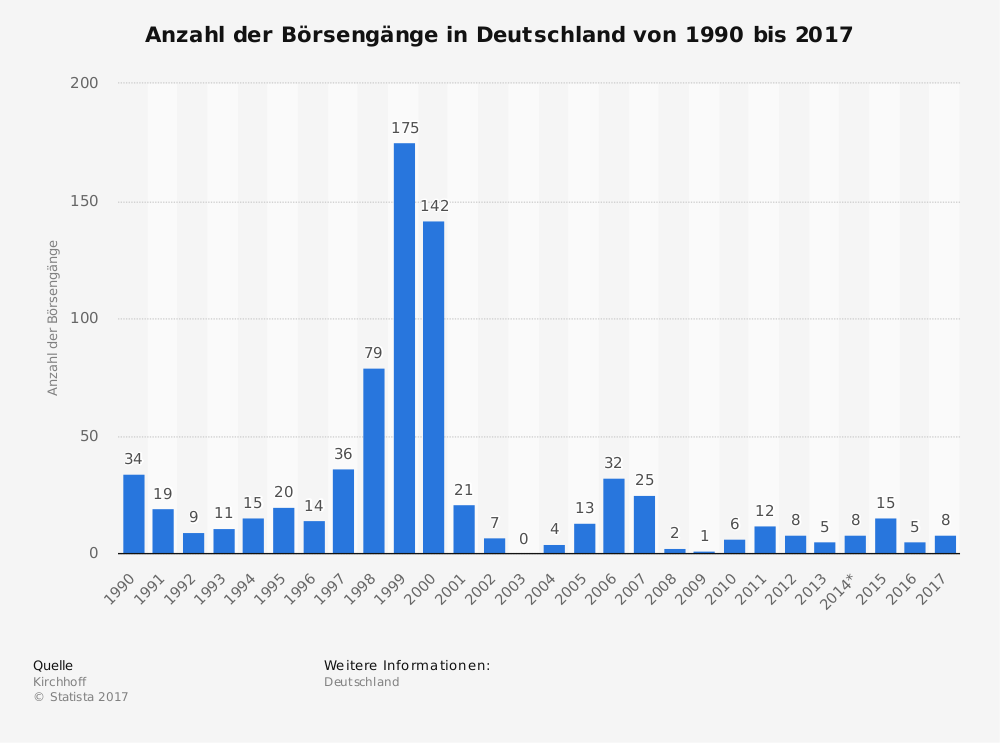
\includegraphics[width=9cm, height=6cm]{anzboersengaenge.PNG}
\end{figure}
\end{frame}

\begin{frame} {Anzahl Börsengänge weltweit 2017 nach Börsen}
\begin{figure}
	\centering
	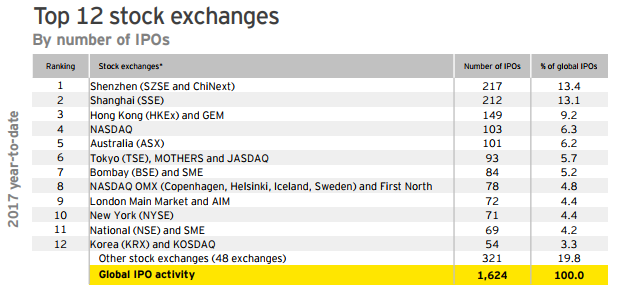
\includegraphics[width=9cm, height=6cm]{anzIPOs2017.PNG}
\end{figure}
\end{frame}

\begin{frame} {Volumen Börsengänge weltweit 2017 nach Börsen}
\begin{figure}
	\centering
	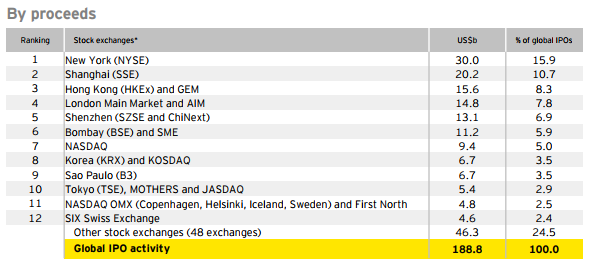
\includegraphics[width=9cm, height=6cm]{IPOsExchangeProceeds.PNG}
\end{figure}
\end{frame}





\subsection{Geschichte von Snap}
\begin{frame} {Was ist Snap Inc.?}
\begin{itemize}
\item Firma mit der Snapchat Software 
\item  Selbstlöschende Bilder
\item  Idee: Reggie Brown und Evan Spiegel
\item  Programmiert: Bobby Murphy
\end{itemize}
\end{frame}

\begin{frame} {Entwicklung}
\begin{itemize}
	\item Zuerst Markenpolitik \pause
	\item  08.05.2012 Reggie Brown Keine Ansprüche von Anteilen der Firma, da keine wertvolle Beiträge zur Entwicklung der App \pause
	\item  24.09.2016 Unternehmen Smapchat Inc. Zu Snap Inc. \pause
	\item  04.2017 Snap an die Börse \pause
	\item 06.2017 Snap Map Teilung des eigenen Standortes \pause
	
\end{itemize}
\end{frame}


\subsection{Gründe für den Einstieg in die Börse}
\begin{frame} {Gründe}
\begin{itemize}
\item Geld für das Wachstums des Unternehmen  \pause
\item Zukauf anderer Firmen oder Expansion auf internationaler Ebene   \pause
\item Empfehlenswert nach allen anderen Geldquellen   \pause
\end{itemize}
\end{frame}
\begin{frame} {Andere Möglichkeiten}
\begin{itemize}
\item Fördermittel oder über Venture-Capital 
\item Fristen und Regeln für die Börsenzulassung
\item Venture-Capital-Gesellschaften und Business Angels
\item Haltung der Anteile nicht für die Ewigkeit
\end{itemize}
\end{frame}



\section{Schluss}
\subsection{Fazit}
\begin{frame}{Fazit}

Snap hat eine richtige/falsche Entscheidung getroffen

\end{frame}



\end{document}